

\documentclass[journal]{IEEEtran}




\usepackage[pdftex]{graphicx}
% \graphicspath{{../pdf/}{../jpeg/}}
% \DeclareGraphicsExtensions{.pdf,.jpeg,.png}
\usepackage{amsmath}
\usepackage{booktabs}
\usepackage{amssymb}
\usepackage{wasysym}
\usepackage{listings}

%\usepackage{algorithmic}
%\usepackage{array}
%\usepackage{url}
% correct bad hyphenation here
\hyphenation{op-tical net-works semi-conduc-tor}

\usepackage{xcolor}
\usepackage{listings}
\lstset{basicstyle=\ttfamily,
	showstringspaces=false,
	commentstyle=\color{red},
	keywordstyle=\color{blue}
}

\usepackage{biblatex}
\usepackage[colorlinks=true,allcolors=black]{hyperref}
%\usepackage[backend=biber, bibencoding=utf8, style=ieee]{biblatex}
\addbibresource{references.bib}






\hyphenation{op-tical net-works semi-conduc-tor}


\begin{document}

\title{Assignment 3 - Phase 2: Using gem5 for estimating the performance of different application mappings onto different multi-core processors
}

\author{Snorri Steffanson, Filippo Bernardi,~\IEEEmembership{Master students,~TU Eindhoven}
}



% The paper headers
\markboth{Using gem5 to simulate application mapped onto different multi-core processors - S. Steffanson, F. Bernardi}%
{Shell \MakeLowercase{\textit{et al.}}: Bare Demo of IEEEtran.cls for IEEE Journals}


\maketitle

% As a general rule, do not put math, special symbols or citations
% in the abstract or keywords.
\begin{abstract}
Performance evaluation of an application mapped onto multiple cores. The application is ray tracing. The CPU setups used are; ARM A15 and ARM A9 and triple ARM A9 cores. The program it has been divided used a profiler but also just by looking at the application itself. 
\end{abstract}

% Note that keywords are not normally used for peerreview papers.
\begin{IEEEkeywords}
ARM A9, ARM A15, GEM5, Pthreads C library, Valgrind, Ray Tracing, Simulation
\end{IEEEkeywords}


\IEEEpeerreviewmaketitle

\section{Introduction}

\IEEEPARstart{T}{his} paper shows performance evaluation of an application, ray tracing\footnote{\hyperref{https://en.wikipedia.org/wiki/Ray_tracing_(graphics)}{}{Ray Tracing}{Wiki page for Ray Tracing}}, onto two different multiprocessor setup. Those two setups are composed firstly there are three ARM A9 core CPUs. The second one has an ARM A15 and an ARM A9 core.
To describe the difference first one has three as powerful balanced cores but the later has one more powerful, the A15, and one A9.
The first step was to analyze the given process. For this task Valgrind was used.
The initial results is shown in figure \ref{fig:valgrind}.

\begin{figure}[!h]
	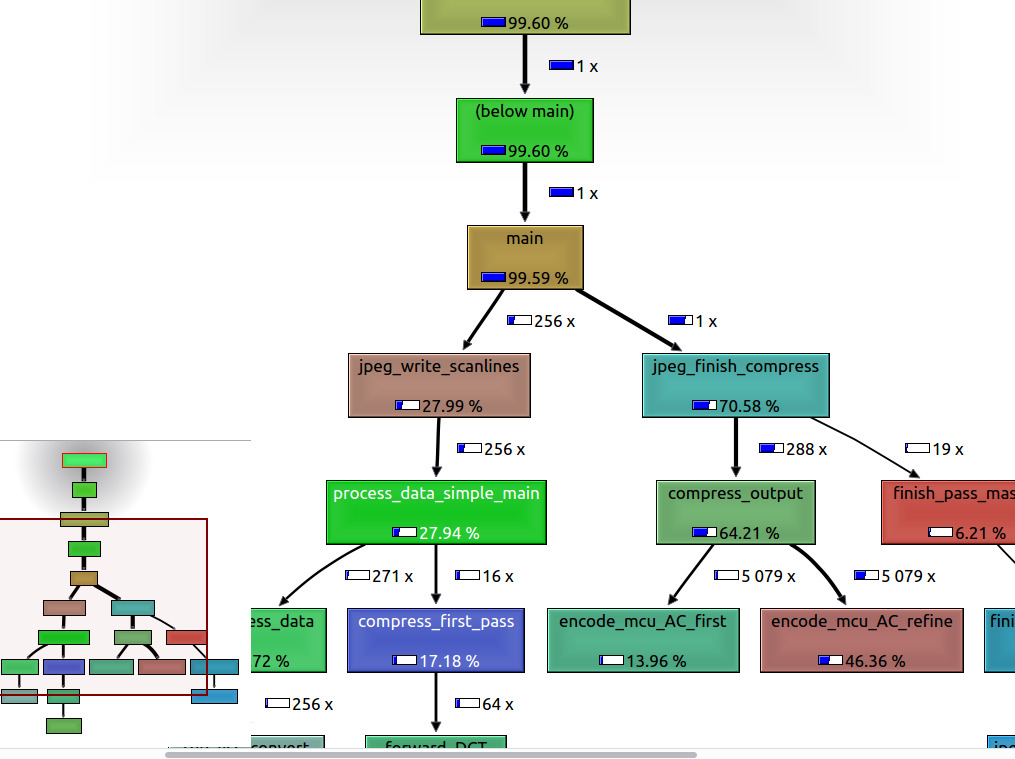
\includegraphics[width=\linewidth]{valgrind}
	\caption{Program calls in Valgrind}
	\label{fig:valgrind}
\end{figure} 

This results gives the hint of how to divide the code onto the different cores and CPU architecture. This paper is divided onto two main sections, the first part concerning the Gem5 simulator and the Pthread library. The other section explains and evaluates result of using those tools and how it was done.\\

 
\hfill January 27, 2017


\section{Gem5 and Pthread library}
\subsection{Gem5 simulator}
Gem5 is a simulator, here used to simulate the different CPU architectures. The effectiveness and the results of the changes made on the code can be observed when running the code on the architectures with different modifications. 

The metric for evaluating the performances are so called "ticks". Ticks are the results that gem5 displays after every simulation and represent the total execution time in picoseconds on the simulated hardware.
 
The simulator can both work in Full System mode and Syscall Emulation mode \(SE mode\). On one hand, in Full System mode the system it is much more accurate but it requires also a higher amount of time for run the simulation, in this case it is possible to boot an entire OS from scratch. On the other hand, in \(SE mode\) the system is less accurate but is much faster were it does not boot the OS, rather uses the host machine.
In this paper the \(SE mode\) is used because it is of interest evaluate an approximate results of the improved performance of this specific process instead of an accurate analysis of the whole system. If making an end product it would be wise to use the Full system mode later on for further enhancements on stability and power consumption.
\subsection{Pthread library}
To divide the code into different threads, the Posix Thread library (pthread) was used.
The library can be used for advanced multi threading with various settings and easy to use API calls. In this assignment, mainly three of these functions were used:

\begin{itemize}
	\item pthread\_create	
\begin{lstlisting}
int pthread_create(pthread_t * thread,
	const pthread_attr_t * attr,
	void * (*start_routine)(void *), 
	void *arg);
\end{lstlisting}
This function is needed to create new thread and the input into this function are constructed as follows:
\begin{itemize}
	\item The variable \(thread\) returns the thread ID. 
	\item \(Attr\) it is possible to gives different attribute to the thread, but set to NULL by default.
	\item \(*start\_routine\) is the pointer to a function which contains the commands which run on the thread. 
	\item \(*arg\) is the argument to pass to the function. In order to pass multiple arguments, it is needed to create a structure, struct, and pass the struct as it has been done later on the report.\\
\end{itemize}

	\item pthread\_join
\begin{lstlisting}
int pthread_join(pthread_t th, 
	void **thread_return);
\end{lstlisting}
In this function a thread is suspended until \(th\) terminates. \(thread\_return\) returns from the function.
This function is used in order to wait until the specific thread has finished executing.
	\item pthread\_exit
\begin{lstlisting}
void pthread_exit(void *retval);
\end{lstlisting}
This terminates a thread, where \(*retval\) returns the value of the function.
\end{itemize}
This description was reviewed from:\\
 \(http://www.yolinux.com/\)



\section{Optimizing Using Threads}

There were two applications used but the first one was aborted due to large and very spread code size. It was difficult to enhance and work with that code. Some progress was made for that application as can be seen in Subsection \ref{sec:jpeg}

\subsection{JPEG - First application}
\label{sec:jpeg}
When starting the optimization of the code and putting it onto threads, both architecture were simulated without any change to the code, the results are the following:
23714598000 number of ticks for the triple A9 cores and 18786430000 for the A15 and A9. 
Now, the jpeg finish compression has been placed in another thread, for doing so the following tutorial has been used: http://timmurphy.org/2010/05/04/pthreads-in-c-a-minimal-working-example/

On one thread the jpeg\_finish\_compress there are the same results for 3 a9 23641697000 and 21533576000 for a15-a9


\subsection{Ray Tracing - New application }
Due to the complexity of the jpeg compressing function it was decided to change to a different application but exploited in a simple manner. The new Program calls tree, from valgrind, can seen in Figure \ref{fig:valgrind2}

\begin{figure}[!h]
	\centering
	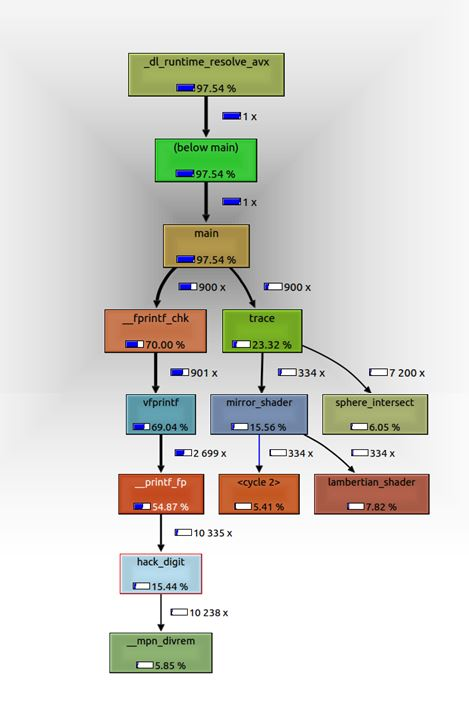
\includegraphics[width=.8\linewidth]{valgrind2}
	\caption{New jpeg application calls in Valgrind}
	\label{fig:valgrind2}
\end{figure}


Valgrind was first used to find the relevant functions to be utilized in threads. That showed that approximately 70\% of the effort went to printing to the image file and 30\% went to the actual tracing. First approach the tracing function and move it to another thread. It sounds like a brilliant idea to have one tread doing the trace but in practice, many changes have to be made in order to do that were for every pixel the function is called. A great overhead would have mean created with that.

Thus next thought was to divided the lines to different threads. Firstly, a thread for each pixels’ line has been created. The idea was to created multiple thread and then let the compiler divide them among all the cores. A thread (one or two) was created and passed any number of threads in any segment of the picture. Ofcourse passing equal amount of pixels(lines) to each thread would make sense but that was not the case. That will be discussed further in the results, in Section \ref{sec:res}.
For doing passing multiple arguments to a thread with pthread\_create a struct had to be defined;
\begin{lstlisting}
struct passToThread_struct{
int width_pixel;
float *res_0T,*res_1T,*res_2T;
scene_t *sceneT;
}f;
\end{lstlisting}
On the main, a normal iteration where left as it was on the code, then a new pixels’ line computation where created. After assign all the variable to pass, the pthread function where invoked:
\begin{lstlisting}
pthread_create(&col_thread_variable[px],
NULL, trace_thread, &f[px]);
\end{lstlisting} 
then the instance 
\begin{lstlisting}
pthread_join(col_thread_variable[px], 
NULL);
\end{lstlisting}
For join the thread to the main one.
The \(trace_thread\) function was created by adapting the code of the main used for calculate a line of pixel.\\

The code was now ready to be run using the script on the appendix.
However, because of gem5 was running in SE mode, it was not possible to create more thread that the cores available and then a different type of code has been created, tailored with the used CPU.
The results can be seen in figure \ref{fig:a9a9a9} for the 3 a9 processor, and in figure \ref{fig:a15a9} for the a15-a9 processor. As it is possible to see the overall performances where decreased of about 1\% and 2\% respectively.
As next step, the picture has been divided equally between the main and another thread. The result where already satisfactory with an increase in performance of 42\% in the 3 A9 processor and 17\% on the A15-A9 processor.\\

Finally, it has been created a different application for the two processors for use as much as possible the available resources. On the A15-A9 processor in fact, it has been allocated more pixel line on the first A15 core more powerful that the secondary A9. Splitting the code in 2/3 and 1/3 respectively for the A15 and A9 core the results was a 23\% of increase in overall performance.
On the other hand, for the triple A9 processor the application was slightly different: because the availability of the three cores, the thread created where three in this case. It has also been seen after some simulation and by printing on screen the order of execution of each pixel line, that the performance increase was much higher if instead of creating a balanced number of pixels’ line into each thread, was quite better to create an unbalanced one. In fact, we allocated 13 line on the first core, 6 on the second and 11 on the third one. The result was 58\% better in performance.





\begin{figure}[!h]
	\centering
	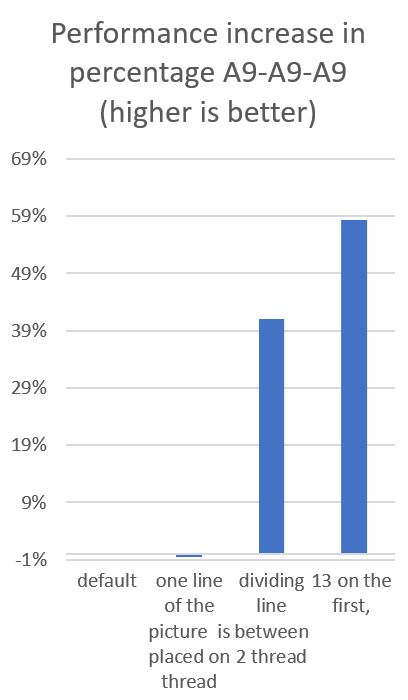
\includegraphics[width=.8\linewidth]{a9a9a9}
	\caption{Performances on a9 a9 a9 processor}
	\label{fig:a9a9a9}
\end{figure}

\begin{figure}[!h]
	\centering
	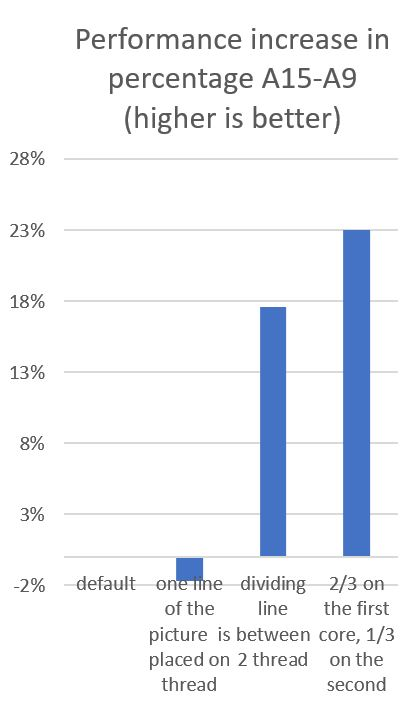
\includegraphics[width=.8\linewidth]{a15a9}
	\caption{Performances on a15 a9 processor}
	\label{fig:a15a9}
\end{figure}

\section{Results and discussion}
\label{sec:res}


\section{appendix}
\subsection{scripts}
\begin{lstlisting}
#!/bin/sh
cd /home/$USER/srt-clean
sudo rm callgrind.out.*
valgrind --tool=callgrind ./srt
kcachegrind callgrind.out.*
cd /
\end{lstlisting}

\begin{lstlisting}
#!/bin/sh
cd /home/$USER/srt-clean
make clean
make
cd /
\end{lstlisting}

\begin{lstlisting}
#!/bin/sh
cd /home/$USER/srt-clean
make clean
make -f Makefile.arm
/home/$USER/gem5/build/ARM/gem5.opt
/home/$USER/gem5/configs/example/arm-multic
	ore-A15-A9.py -c
	/home/$USER/srt-clean/srt
cd /
\end{lstlisting}

\begin{lstlisting}
#!/bin/sh
cd /home/$USER/jpeg/jpeg-6a/
make clean
make -f Makefile.arm
/home/$USER/gem5/build/ARM/gem5.opt
	 /home/$USER/gem5/configs/example/
	arm-multicore-A9-A9-A9.py -c 
	/home/$USER/srt-clean/srt
cd /
\end{lstlisting}


\begin{lstlisting}
#!/bin/sh
cd /home/$USER/srt-clean
make clean
make -f Makefile.arm
cd /
\end{lstlisting}



\section{Conclusion}
It is possible to conclude that the triple A9 has better performance that the A15-A9. This is true depending on how the program is divided onto the three or two cores. Moreover, there are cases where it is not possible to exploit parallelism, in this cases just one core is it used and the A15 one could win due to its characteristic. On the other hand, as in the Jpeg application, where parallelism was possible, it counts more the overall cores power in exploiting better performance. 
\end{document}


